\section{Use Cases}
\label{sec:use_cases}

This section will present the use cases for the system, divided into four actors: system owner, organizer, validator, and user. All of them have similar use case, the authenticate use case, which is responsible for authenticating the users on the system.
On the Subsection \ref{subsec:system_owner_use_cases} we have the use cases for the system owner, where it mentions the management of the system settings and the control of the organizers that have access to the system.
On the Subsection \ref{subsec:organizer_use_cases} we have the use cases for the organizer that mention the creation and management of the events, along with the control of the validators for the event.
On the Subsection \ref{subsec:validator_use_cases} we have the use cases for the validator, and the only thing he can do is to validate the users' tickets.
Lastly, on the Subsection \ref{subsec:user_use_cases} we have the use cases for the common user, like the purchase, gift, refund and resell of tickets.

\subsection{System owner use cases}
\label{subsec:system_owner_use_cases}

As we can see in the Figure \ref{fig:system_owner_use_cases}, the system owner has the specific use case to control event organizers. This is important because the he needs to have control over the organizers that have access to the system. The system owner can also manage the system settings, which is important to control the system's behavior and to adapt it to the organizers' needs.

\begin{figure}[H]
    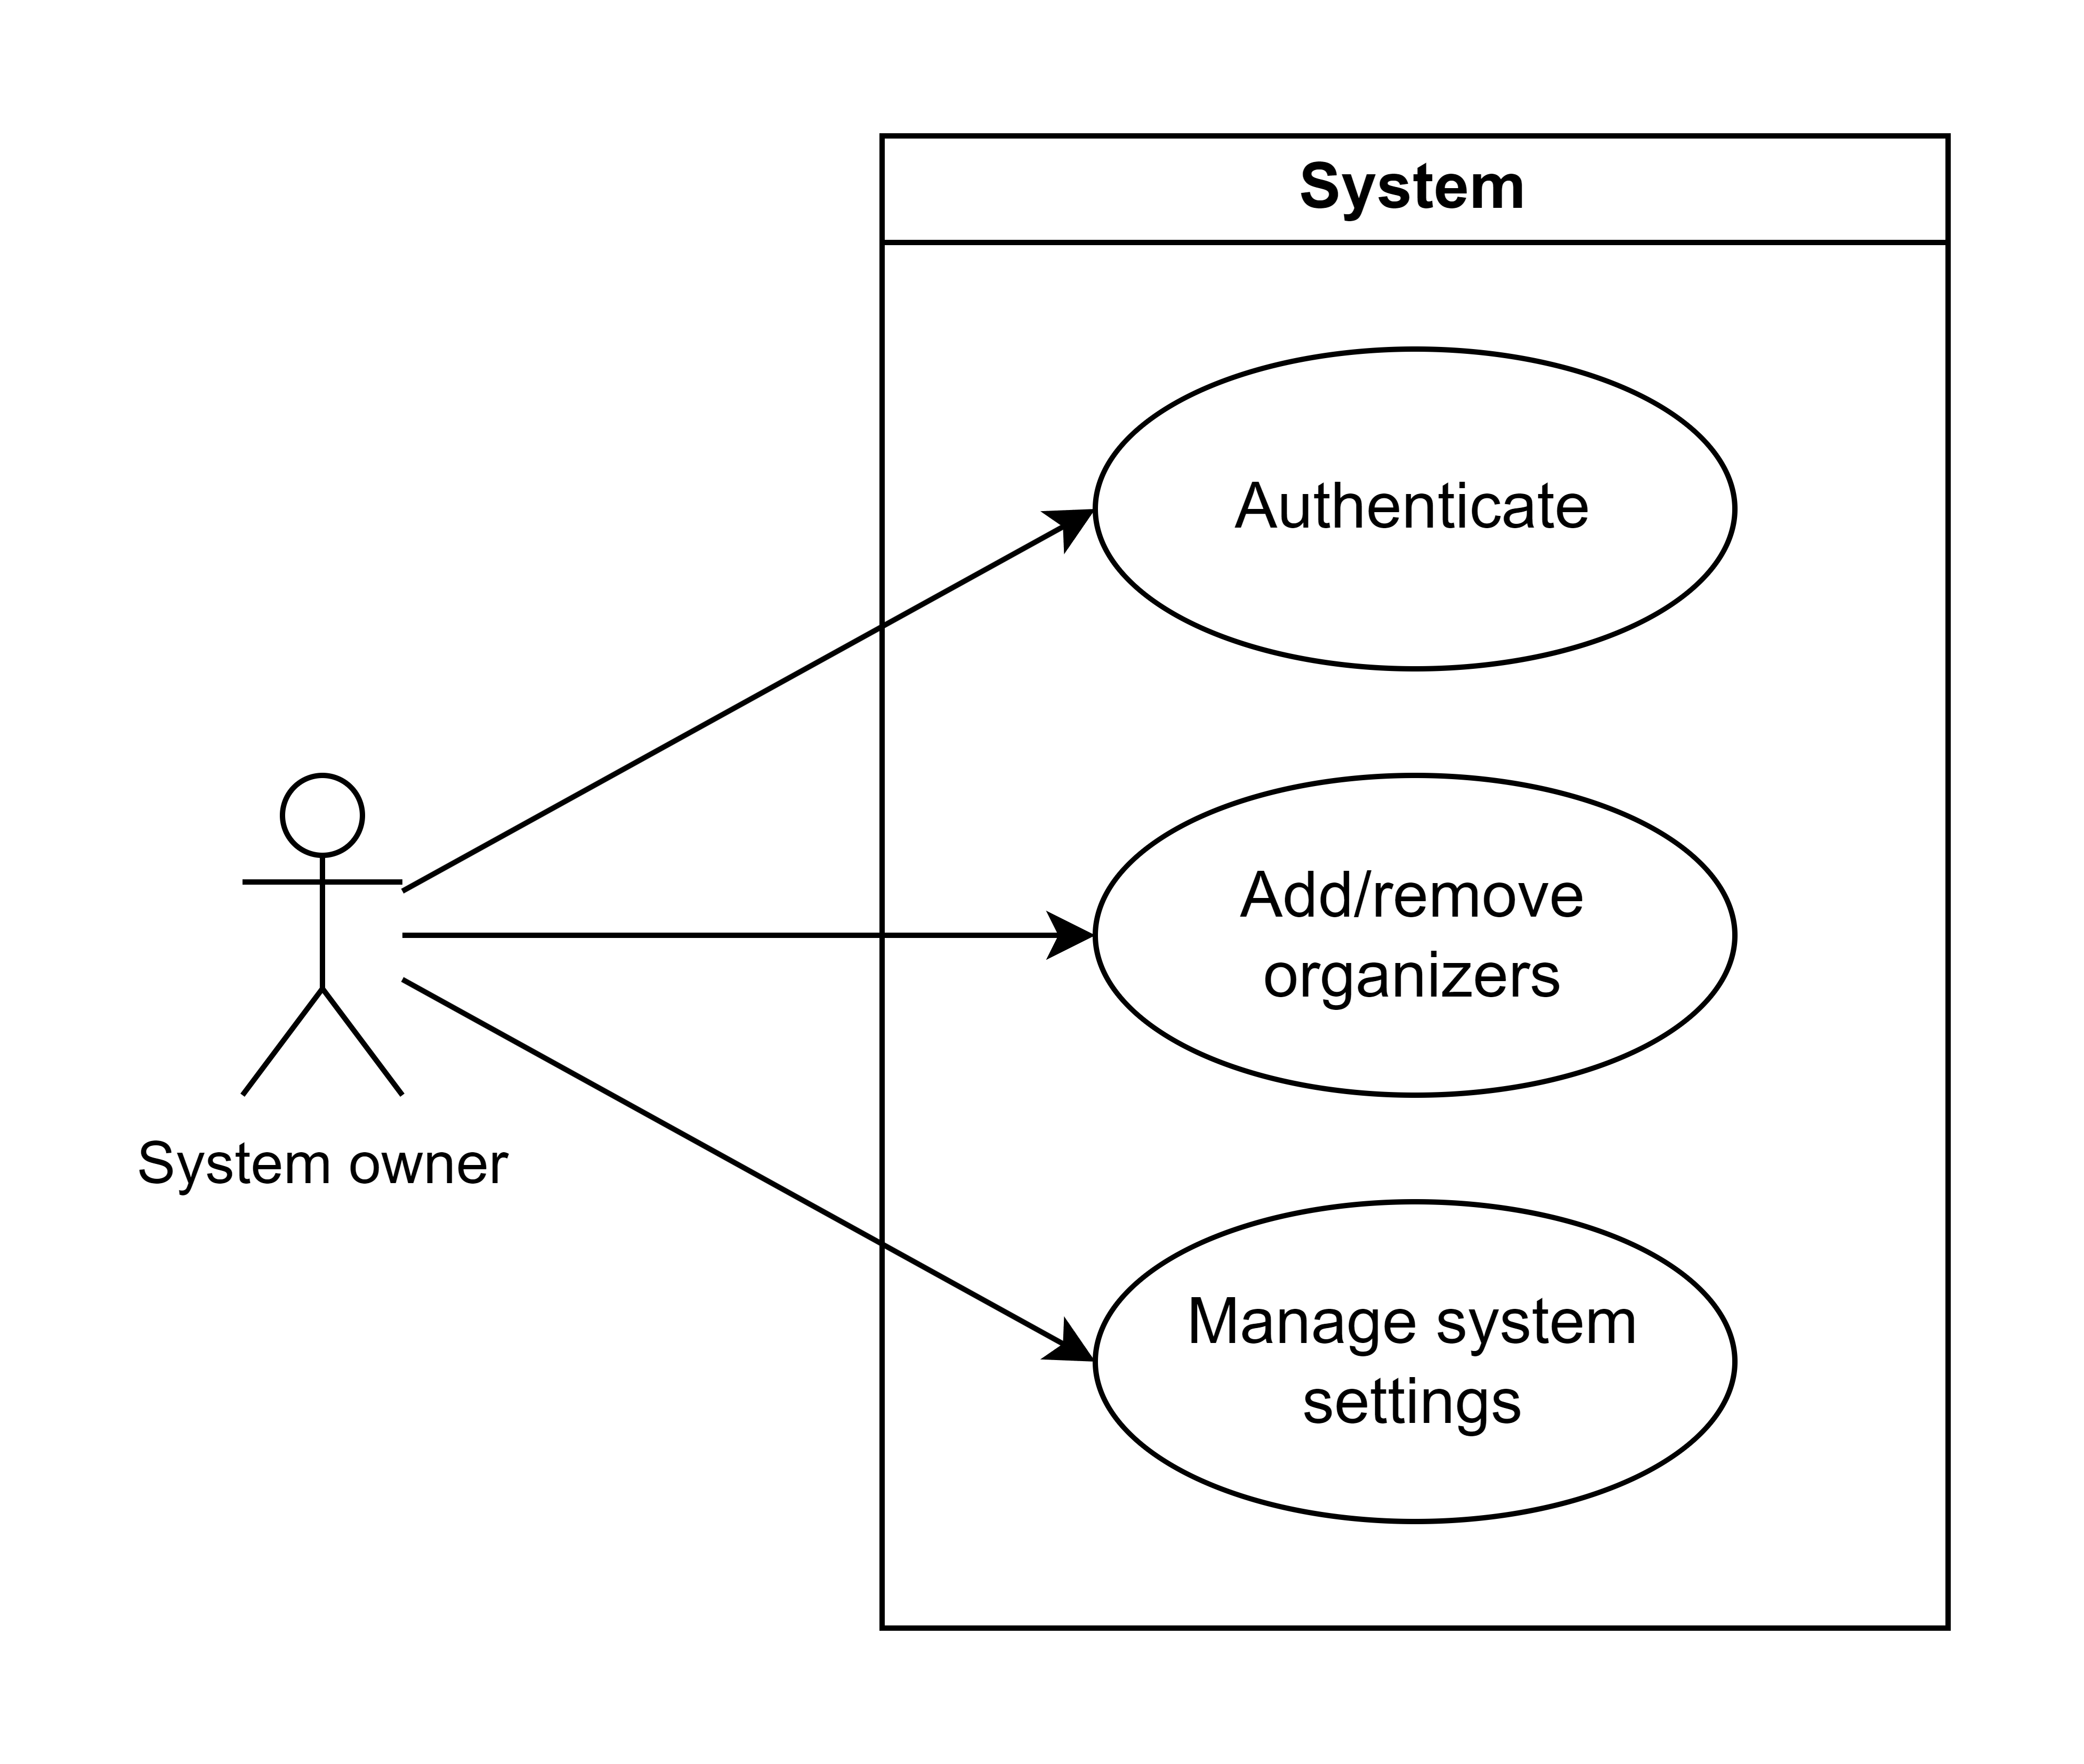
\includegraphics[width=\textwidth/2]{System owner use cases.png}
    \centering
    \caption{System owner use cases}
    \label{fig:system_owner_use_cases}
\end{figure}

\subsection{Organizer use cases}
\label{subsec:organizer_use_cases}

The organizer has the use cases to create events, as we can see in the Figure \ref{fig:organizer_use_cases}. He can also control the validators for the event, which is important to select the people that have the authority to validate the tickets for each event. The organizer can also manage the event settings, like updating the event information or cancel it if really needed.

\begin{figure}[H]
    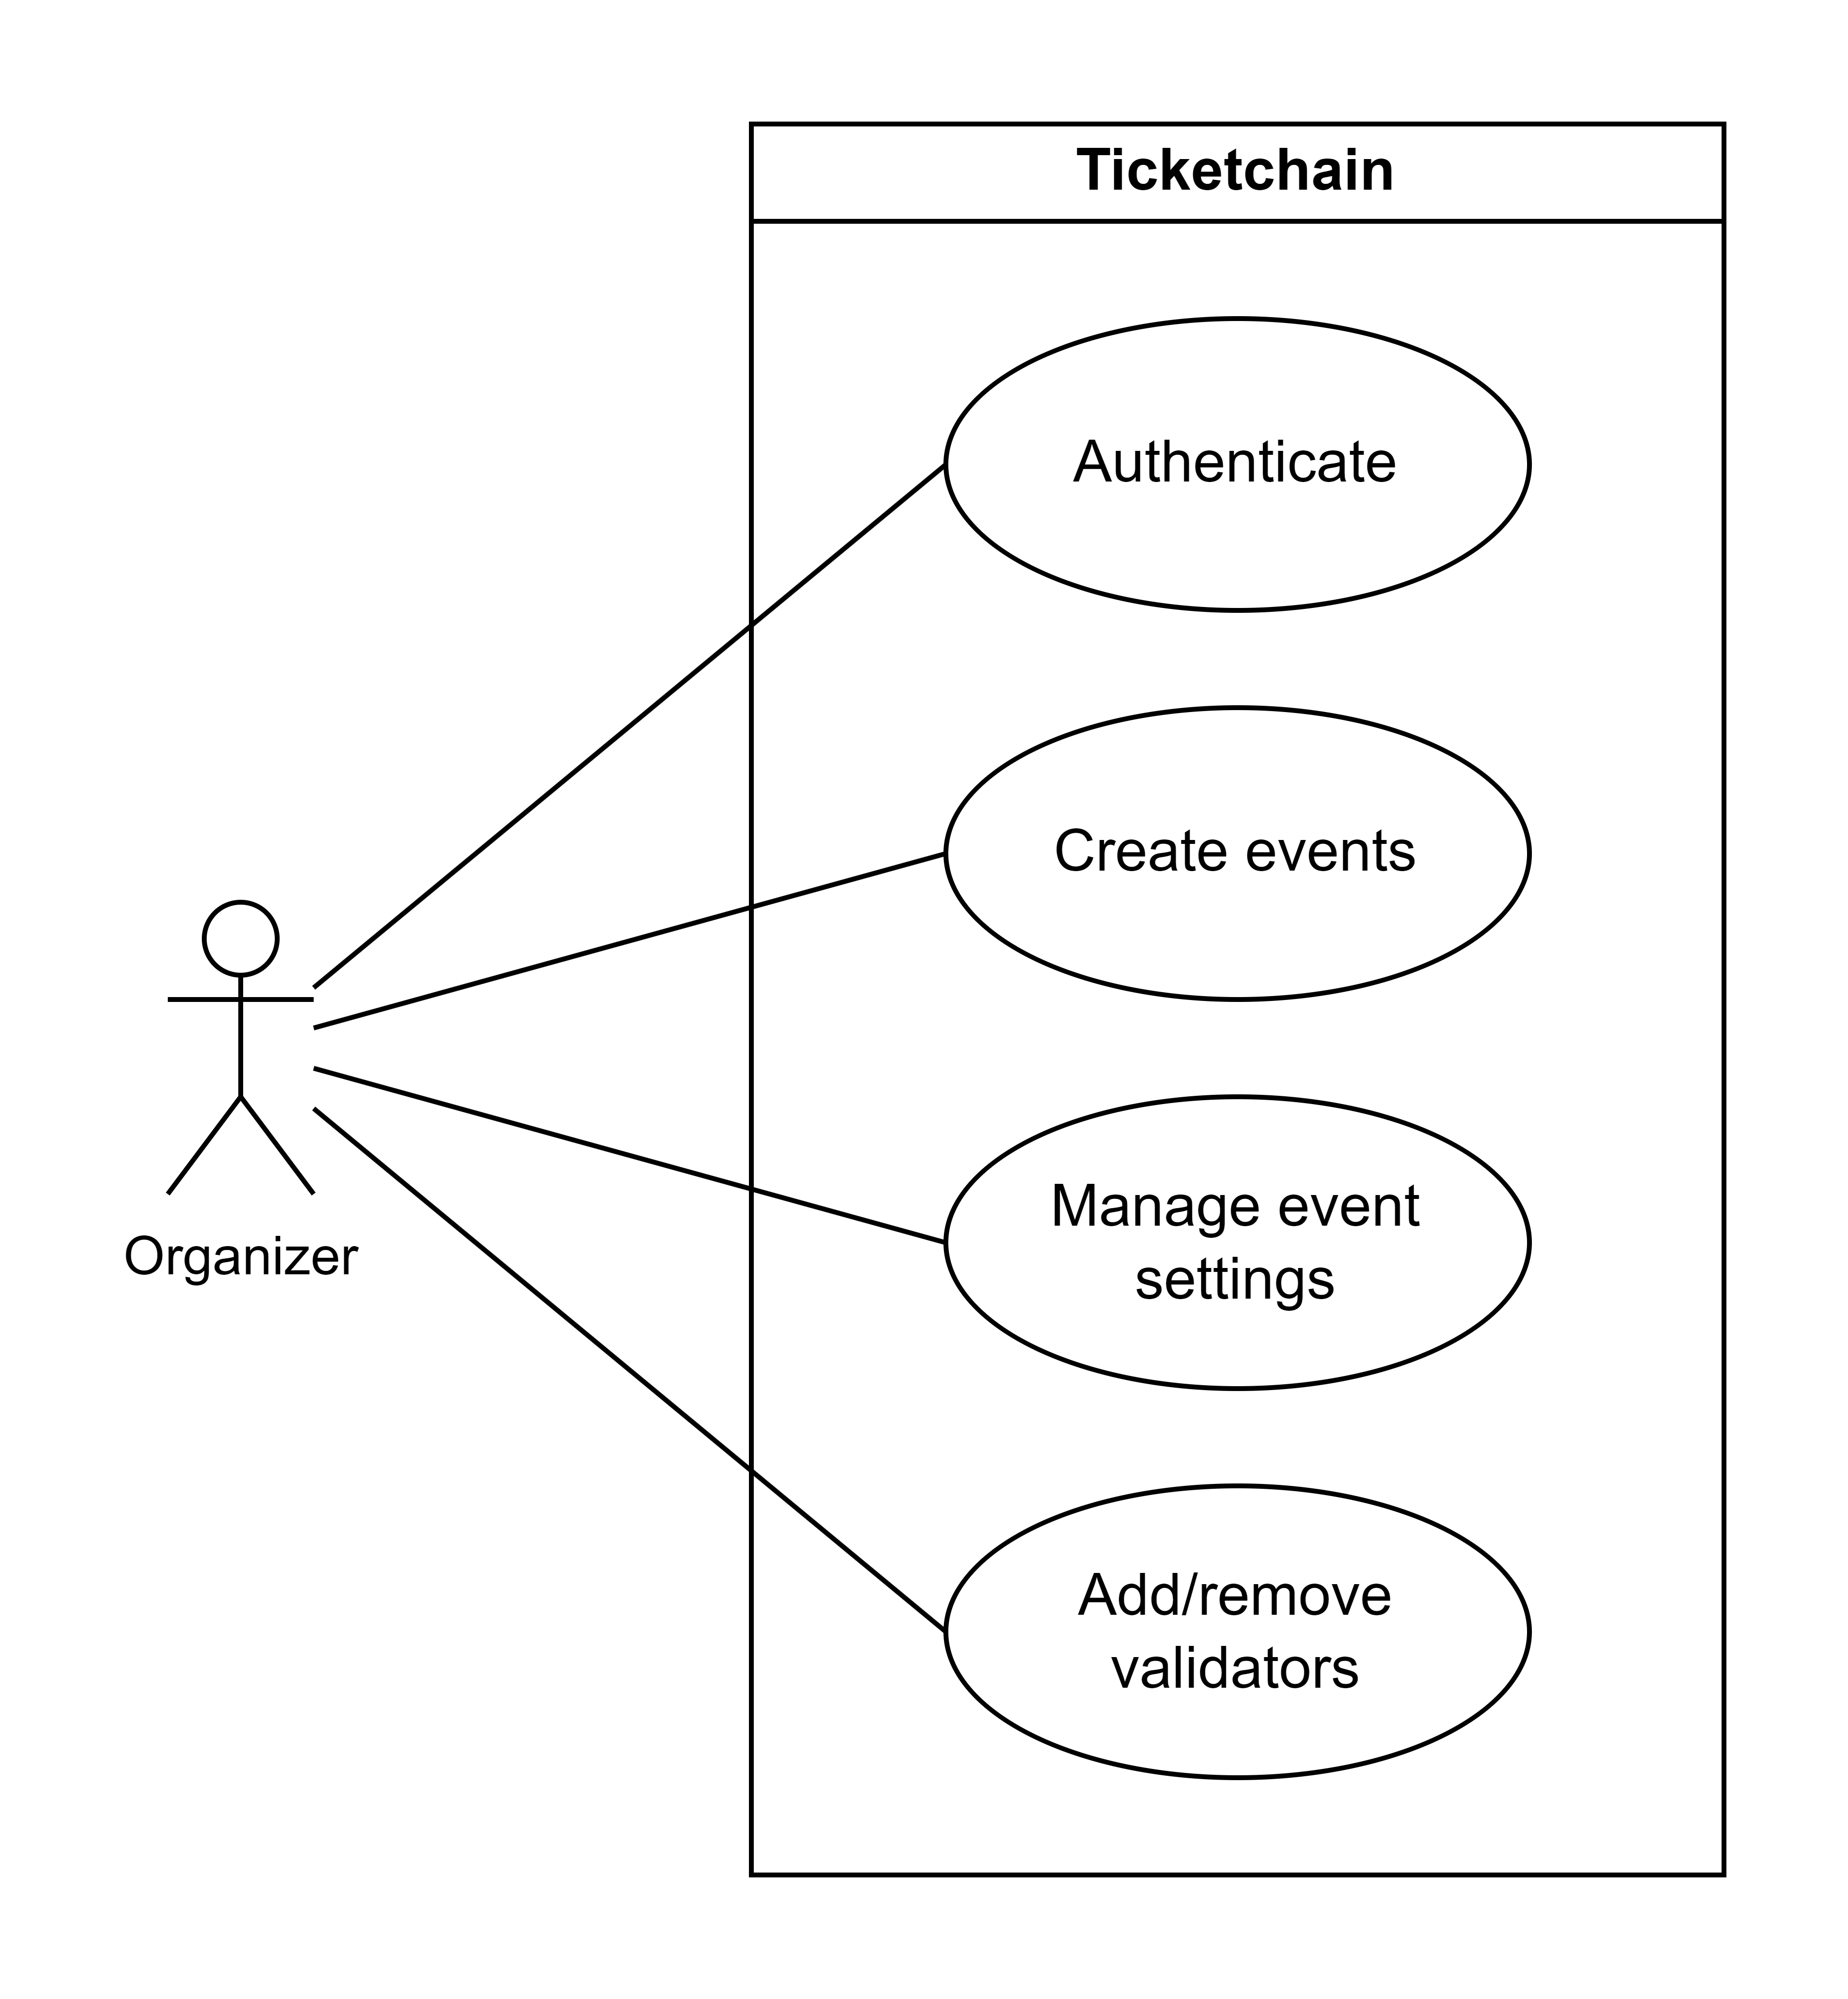
\includegraphics[width=\textwidth/2]{Organizer use cases.png}
    \centering
    \caption{Organizer use cases}
    \label{fig:organizer_use_cases}
\end{figure}

\subsection{Validator use cases}
\label{subsec:validator_use_cases}

For the validators, as we see in the Figure \ref{fig:validator_use_cases}, the only use case is to validate the users' tickets and to allow them to enter the event. This is a necessary step to avoid users to try to bypass this security measure and to ensure that only the users that have a valid ticket can enter the event.

\begin{figure}[H]
    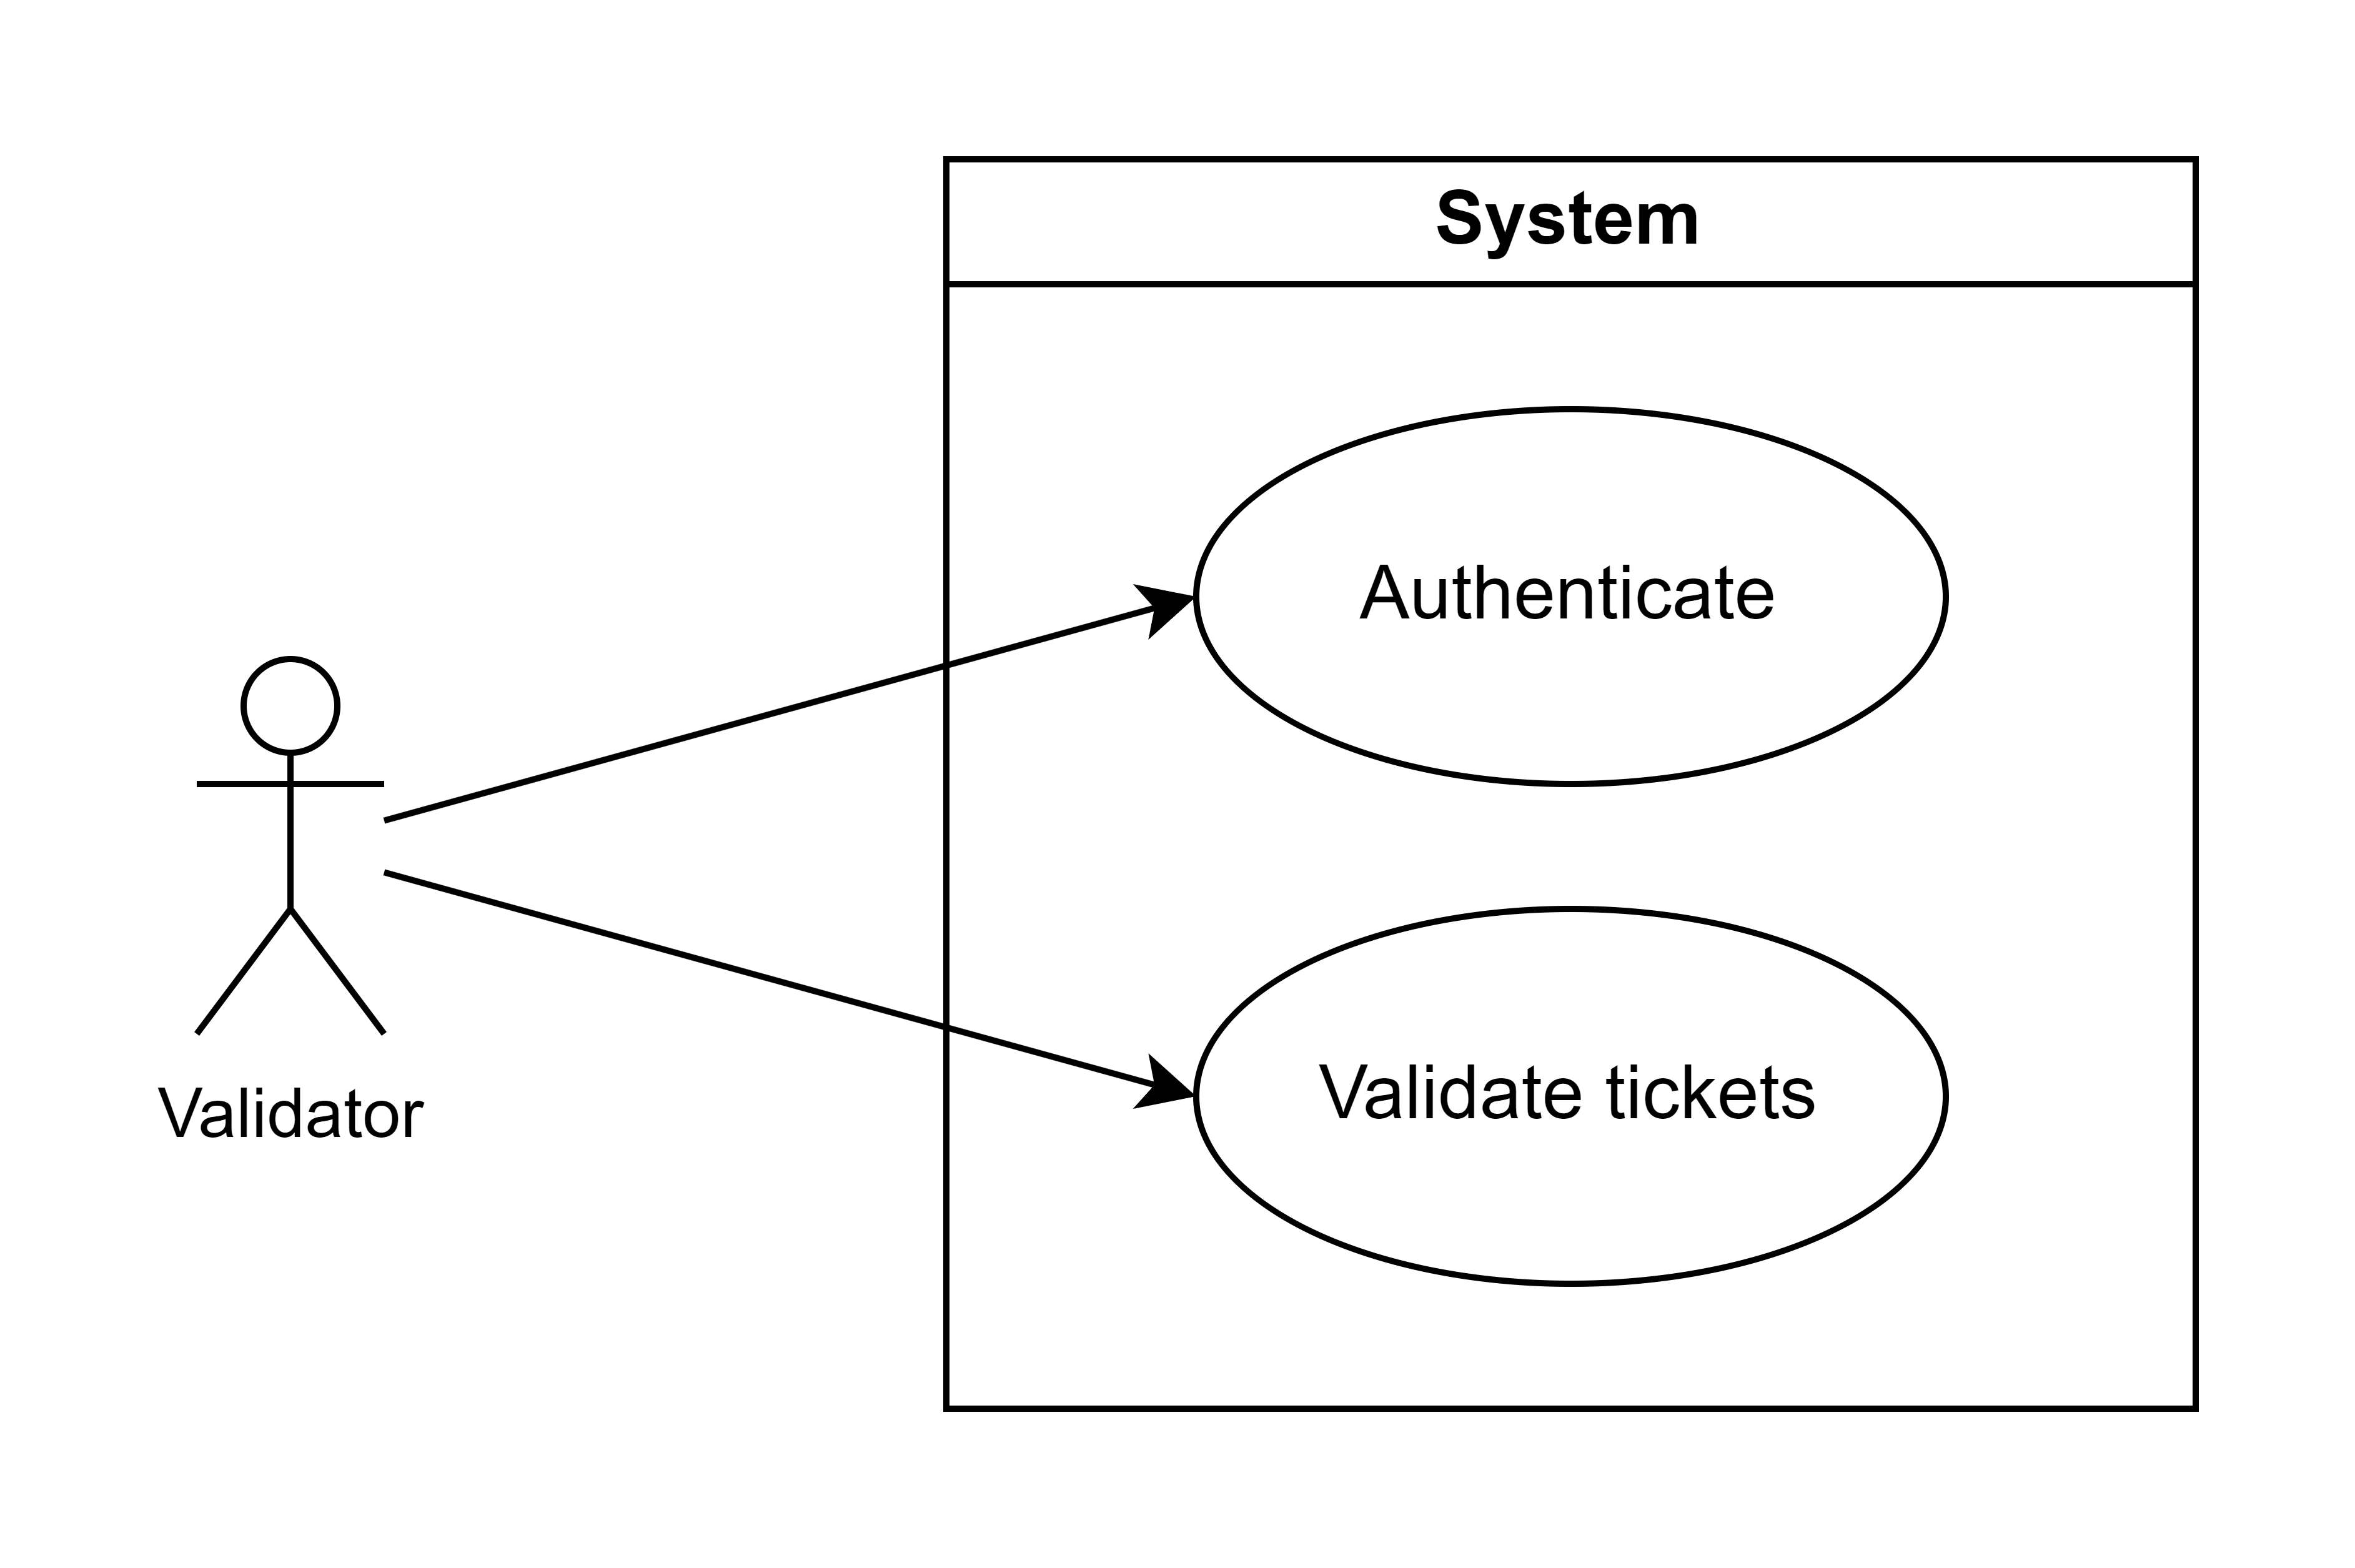
\includegraphics[width=\textwidth/2]{Validator use cases.png}
    \centering
    \caption{Validator use cases}
    \label{fig:validator_use_cases}
\end{figure}

\subsection{User use cases}
\label{subsec:user_use_cases}

In the Figure \ref{fig:user_use_cases} we see the use cases for the common user. The user can purchase tickets for the events, gift tickets to other users, refund tickets if he doesn't want to go to the event anymore (depending on the configuration of the specific event), and resell tickets if he wants to sell them to other users (with the guarantee that he can't sell at a higher price than the original). All of these use cases are important to give the user the flexibility to manage his tickets and have the freedom to do what he wants with them, within the system's rules, of course

\begin{figure}[H]
    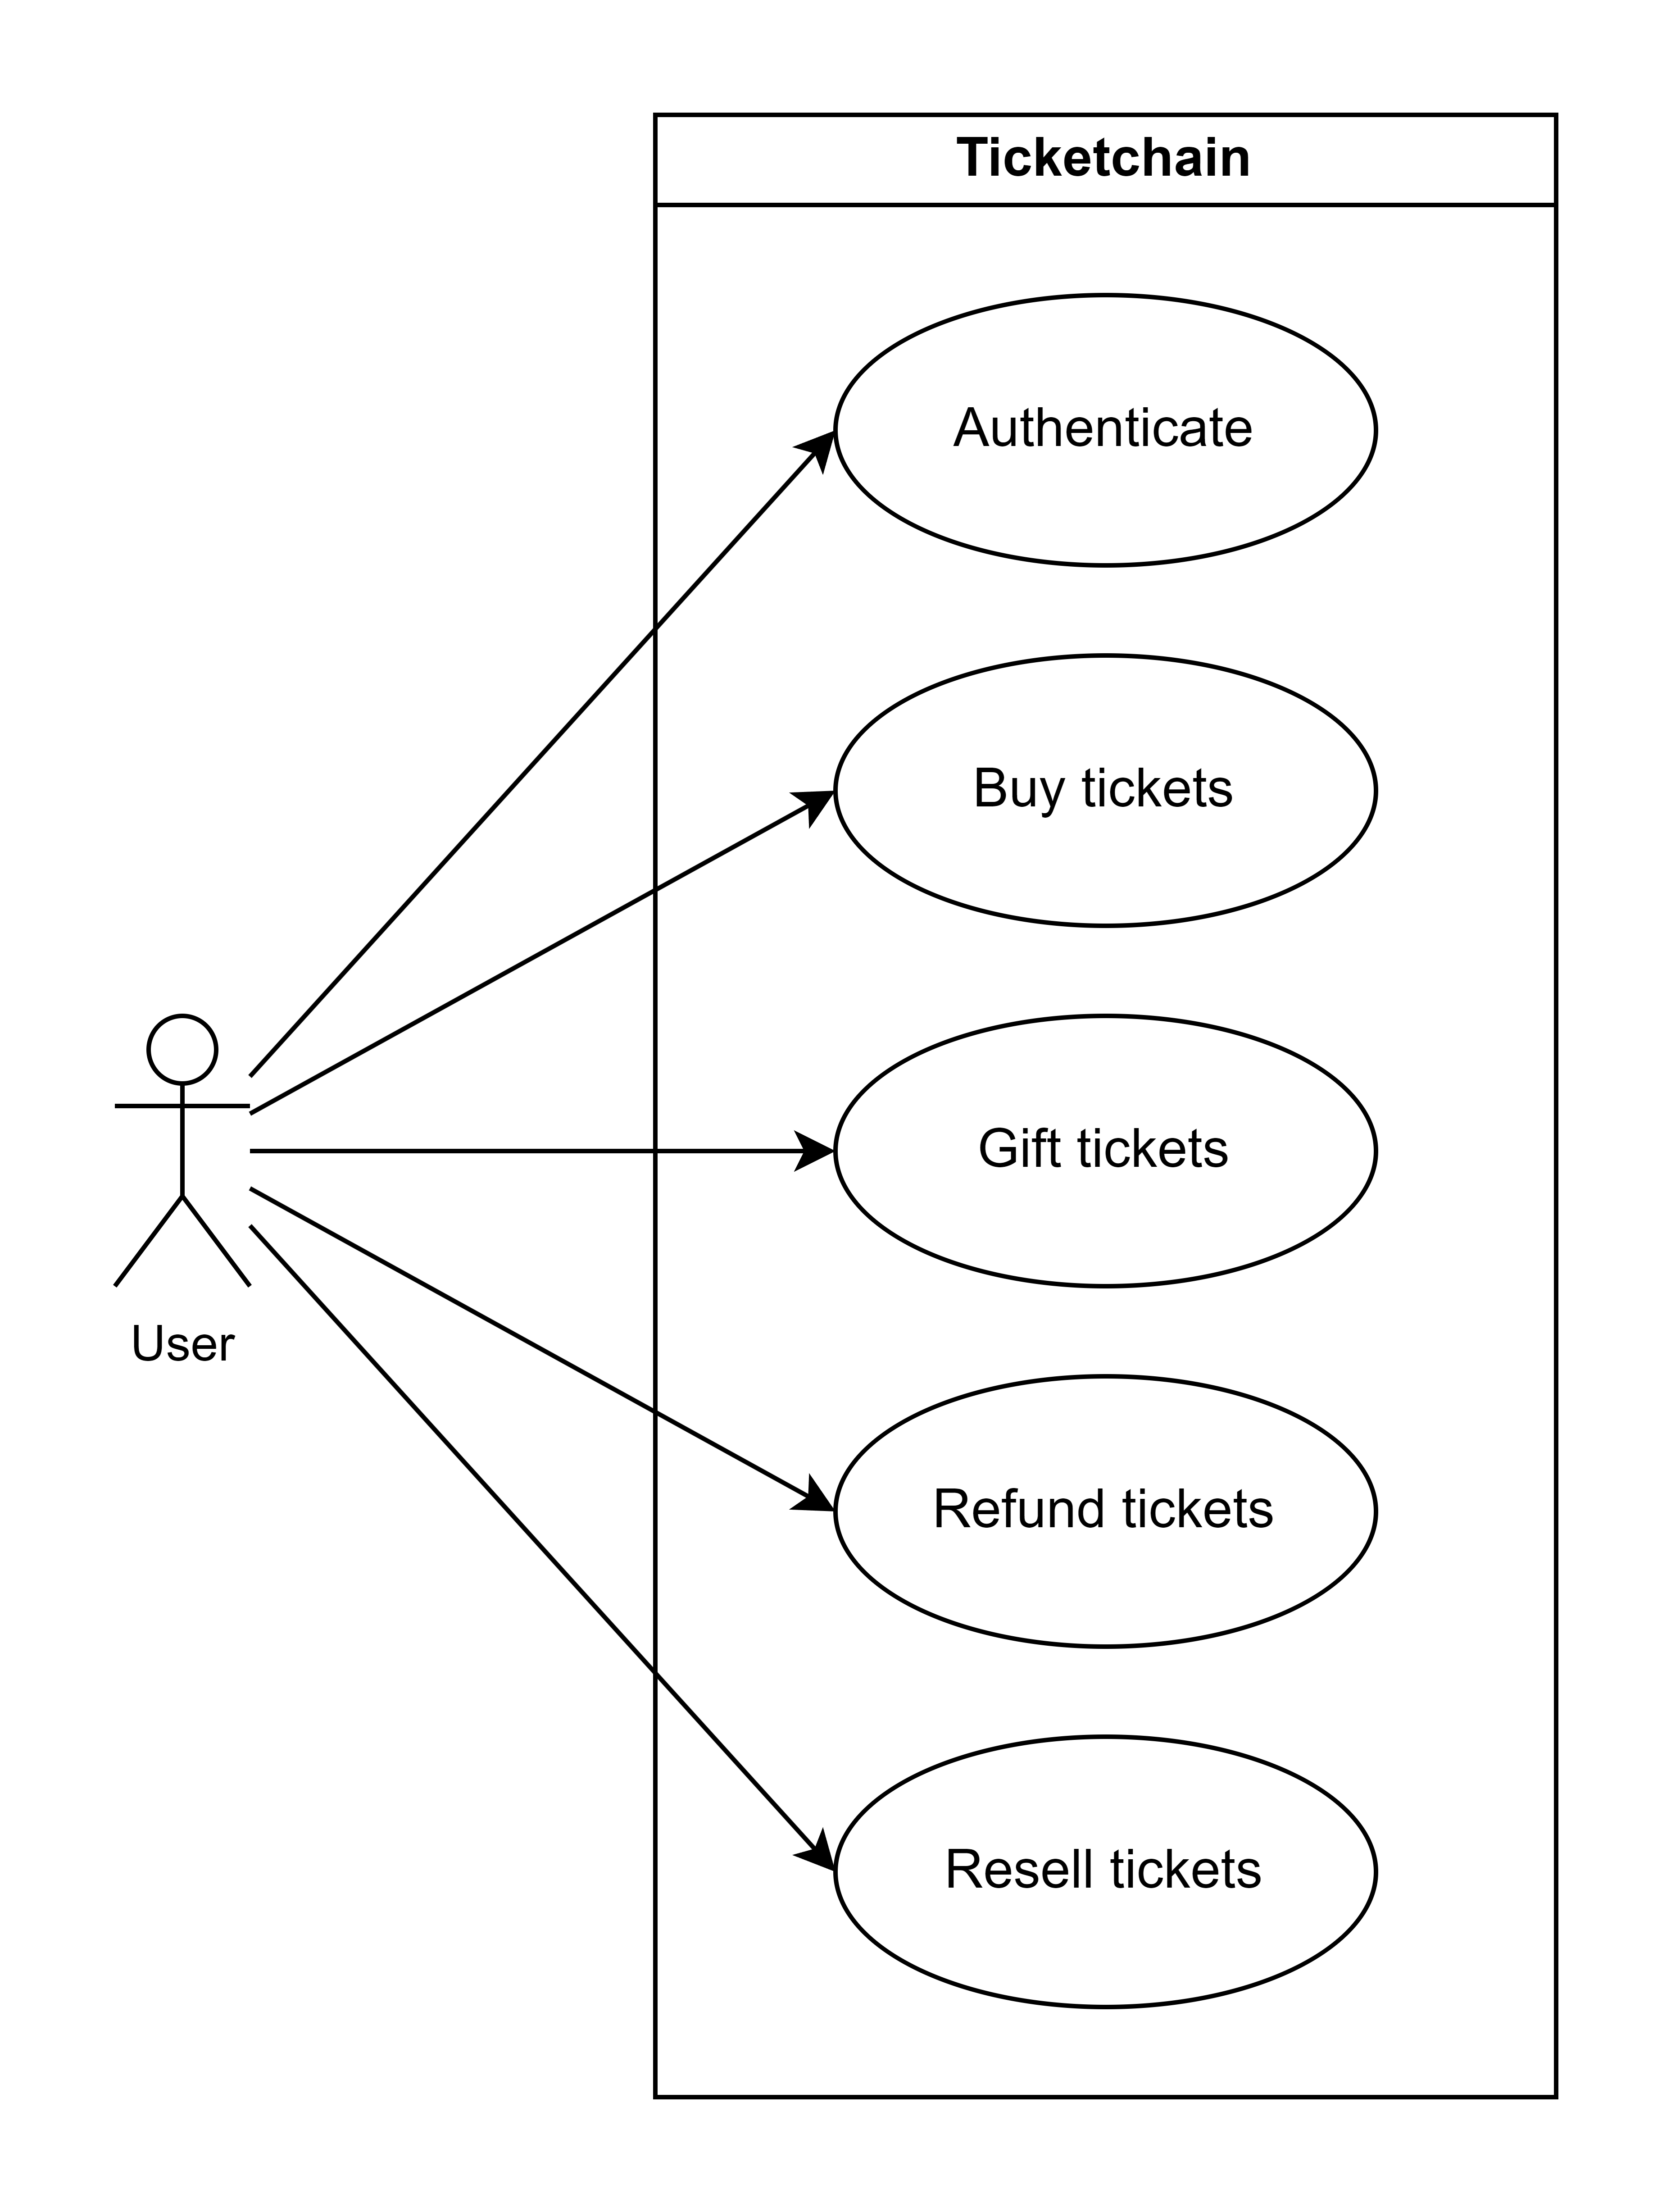
\includegraphics[width=\textwidth/2]{User use cases.png}
    \centering
    \caption{User use cases}
    \label{fig:user_use_cases}
\end{figure}
